% !Mode:: "TeX:UTF-8"
\chapter{实验结果与分析}

本章呈现全部七组实验的结果，并进行系统性分析。所有数据均以权威实验索引为准。

\section{VerilogEval-Human基线实验}

本节报告中期阶段在VerilogEval-Human 20题子集上使用Haiku模型的基线实验结果。

\subsection{总体结果}

\begin{table}[htbp]
\centering
\caption{VerilogEval-Human 20题基线实验结果}
\label{tab:verilogeval_baseline}
\begin{tabular}{lrr}
\toprule
条件 & 通过数 & 通过率 \\
\midrule
Zero-shot & 16/20 & 80\% \\
Feedback & 18/20 & 90\% \\
提升 & +2 & +10个百分点 \\
\bottomrule
\end{tabular}
\end{table}

反馈循环将通过率从80\%提升至90\%。在4道零样本失败的题目中，反馈成功修复了2道（50\%）。

\begin{figure}[htbp]
\centering
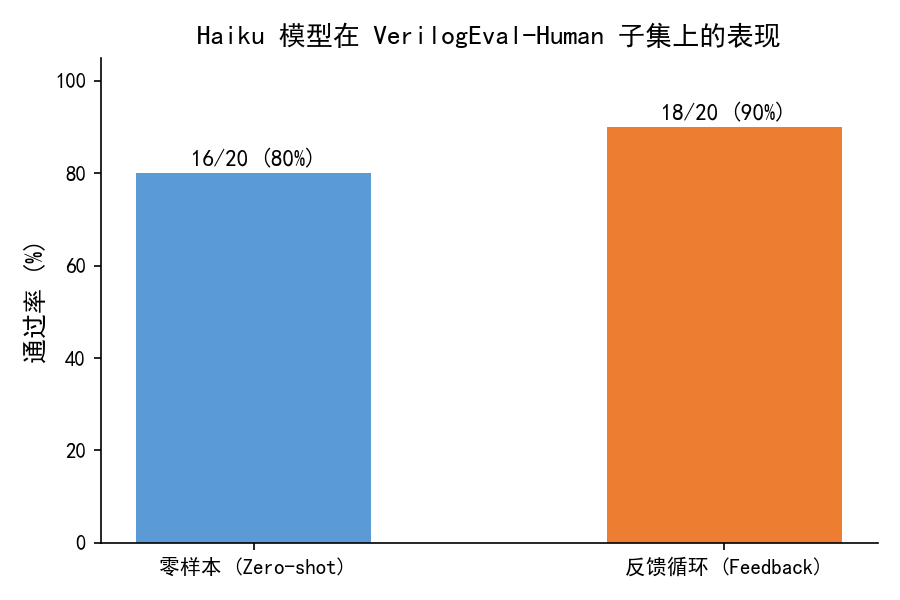
\includegraphics[width=0.7\textwidth]{figure/haiku_pass_rate_bar.png}
\caption{VerilogEval-Human 20题零样本与反馈通过率对比}
\label{fig:verilogeval_bar}
\end{figure}

\subsection{改善与失败案例}

反馈成功修复的两道题为Prob109\_fsm1和Prob127\_lemmings1，均属于"代码接近正确但存在局部状态转移错误"的场景。反馈未能修复的两道题为Prob082\_lfsr32（LFSR抽头多项式属于精确数学知识）和Prob140\_fsm\_hdlc（HDLC协议边界条件极为复杂）。

\subsection{小结}

VerilogEval-Human基线实验初步验证了反馈循环的有效性：对局部逻辑错误修复效果明显，但对领域知识缺口和深层协议逻辑改善有限。

\section{RTLLM\_STUDY\_12正式实验结果}

\subsection{总体结果}

在RTLLM\_STUDY\_12上使用三个模型进行Zero-shot与Feedback对比，结果如表\ref{tab:formal_results}所示。

\begin{table}[htbp]
\centering
\caption{RTLLM\_STUDY\_12三模型正式实验结果}
\label{tab:formal_results}
\begin{tabular}{lrrrr}
\toprule
模型 & Zero-shot & Feedback & 提升 & 改善题数 \\
\midrule
Haiku 4.5 & 5/12 (42\%) & 6/12 (50\%) & +8pp & 2 \\
Sonnet 4.6 & 5/12 (42\%) & 7/12 (58\%) & +17pp & 2 \\
GPT-5.4 & 6/12 (50\%) & 10/12 (83\%) & +33pp & 4 \\
\bottomrule
\end{tabular}
\end{table}

三组实验的API错误率均为零。

\begin{figure}[htbp]
\centering
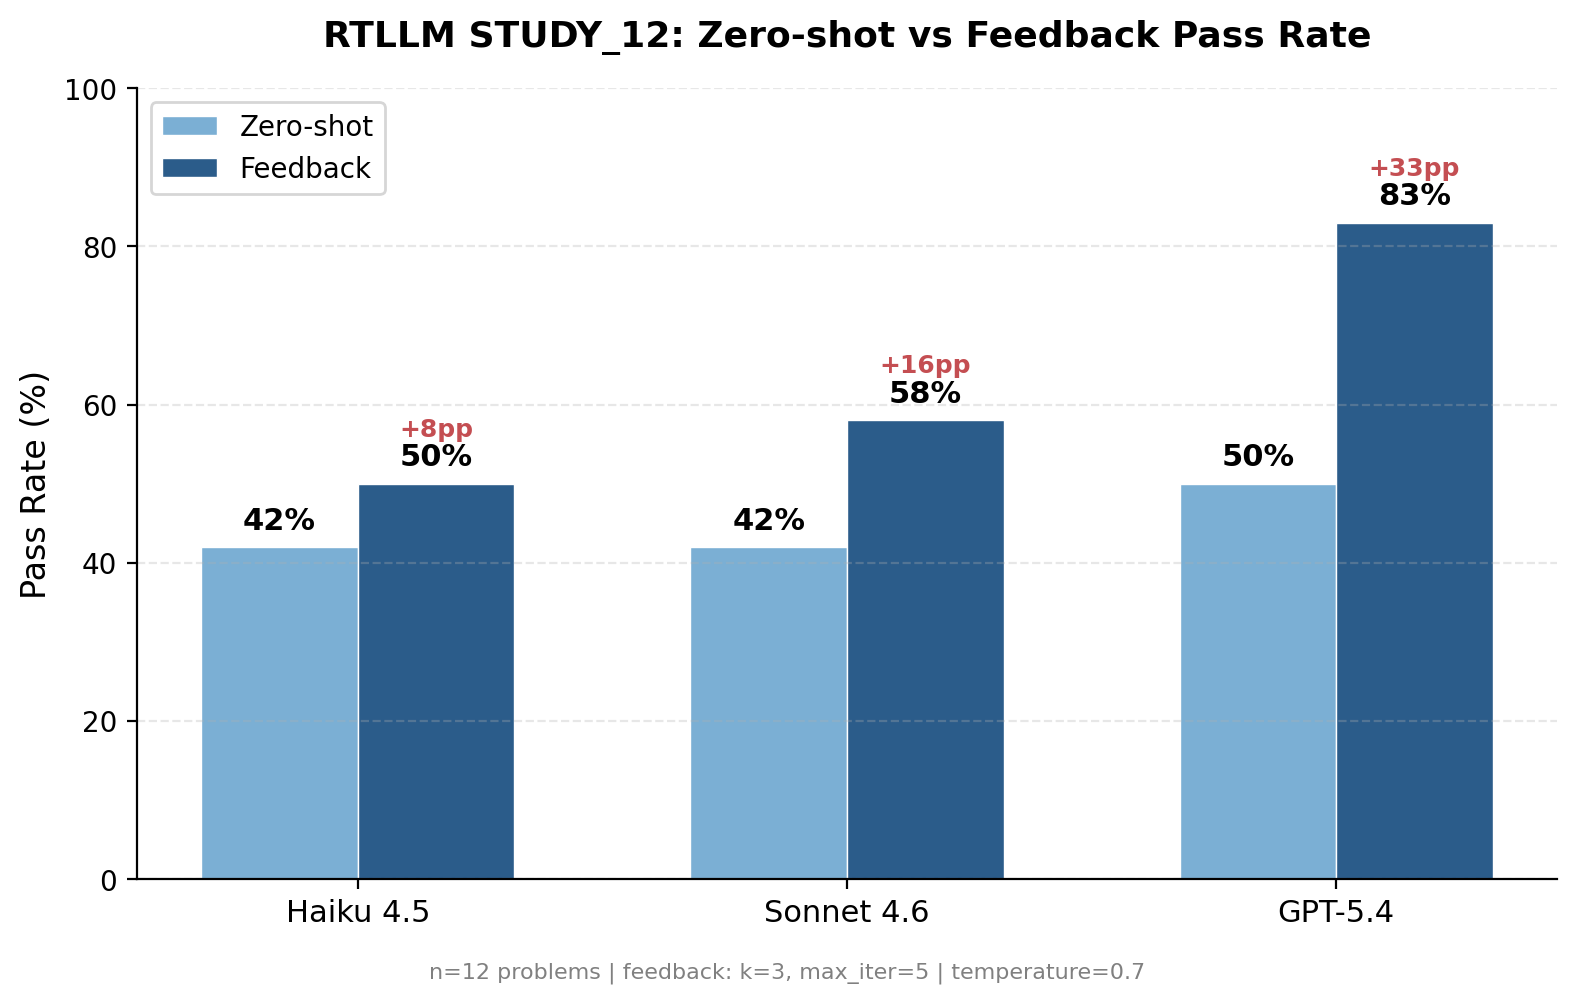
\includegraphics[width=0.7\textwidth]{figure/fig_passrate_comparison.png}
\caption{RTLLM\_STUDY\_12三模型通过率对比}
\label{fig:passrate_comparison}
\end{figure}

\begin{figure}[htbp]
\centering
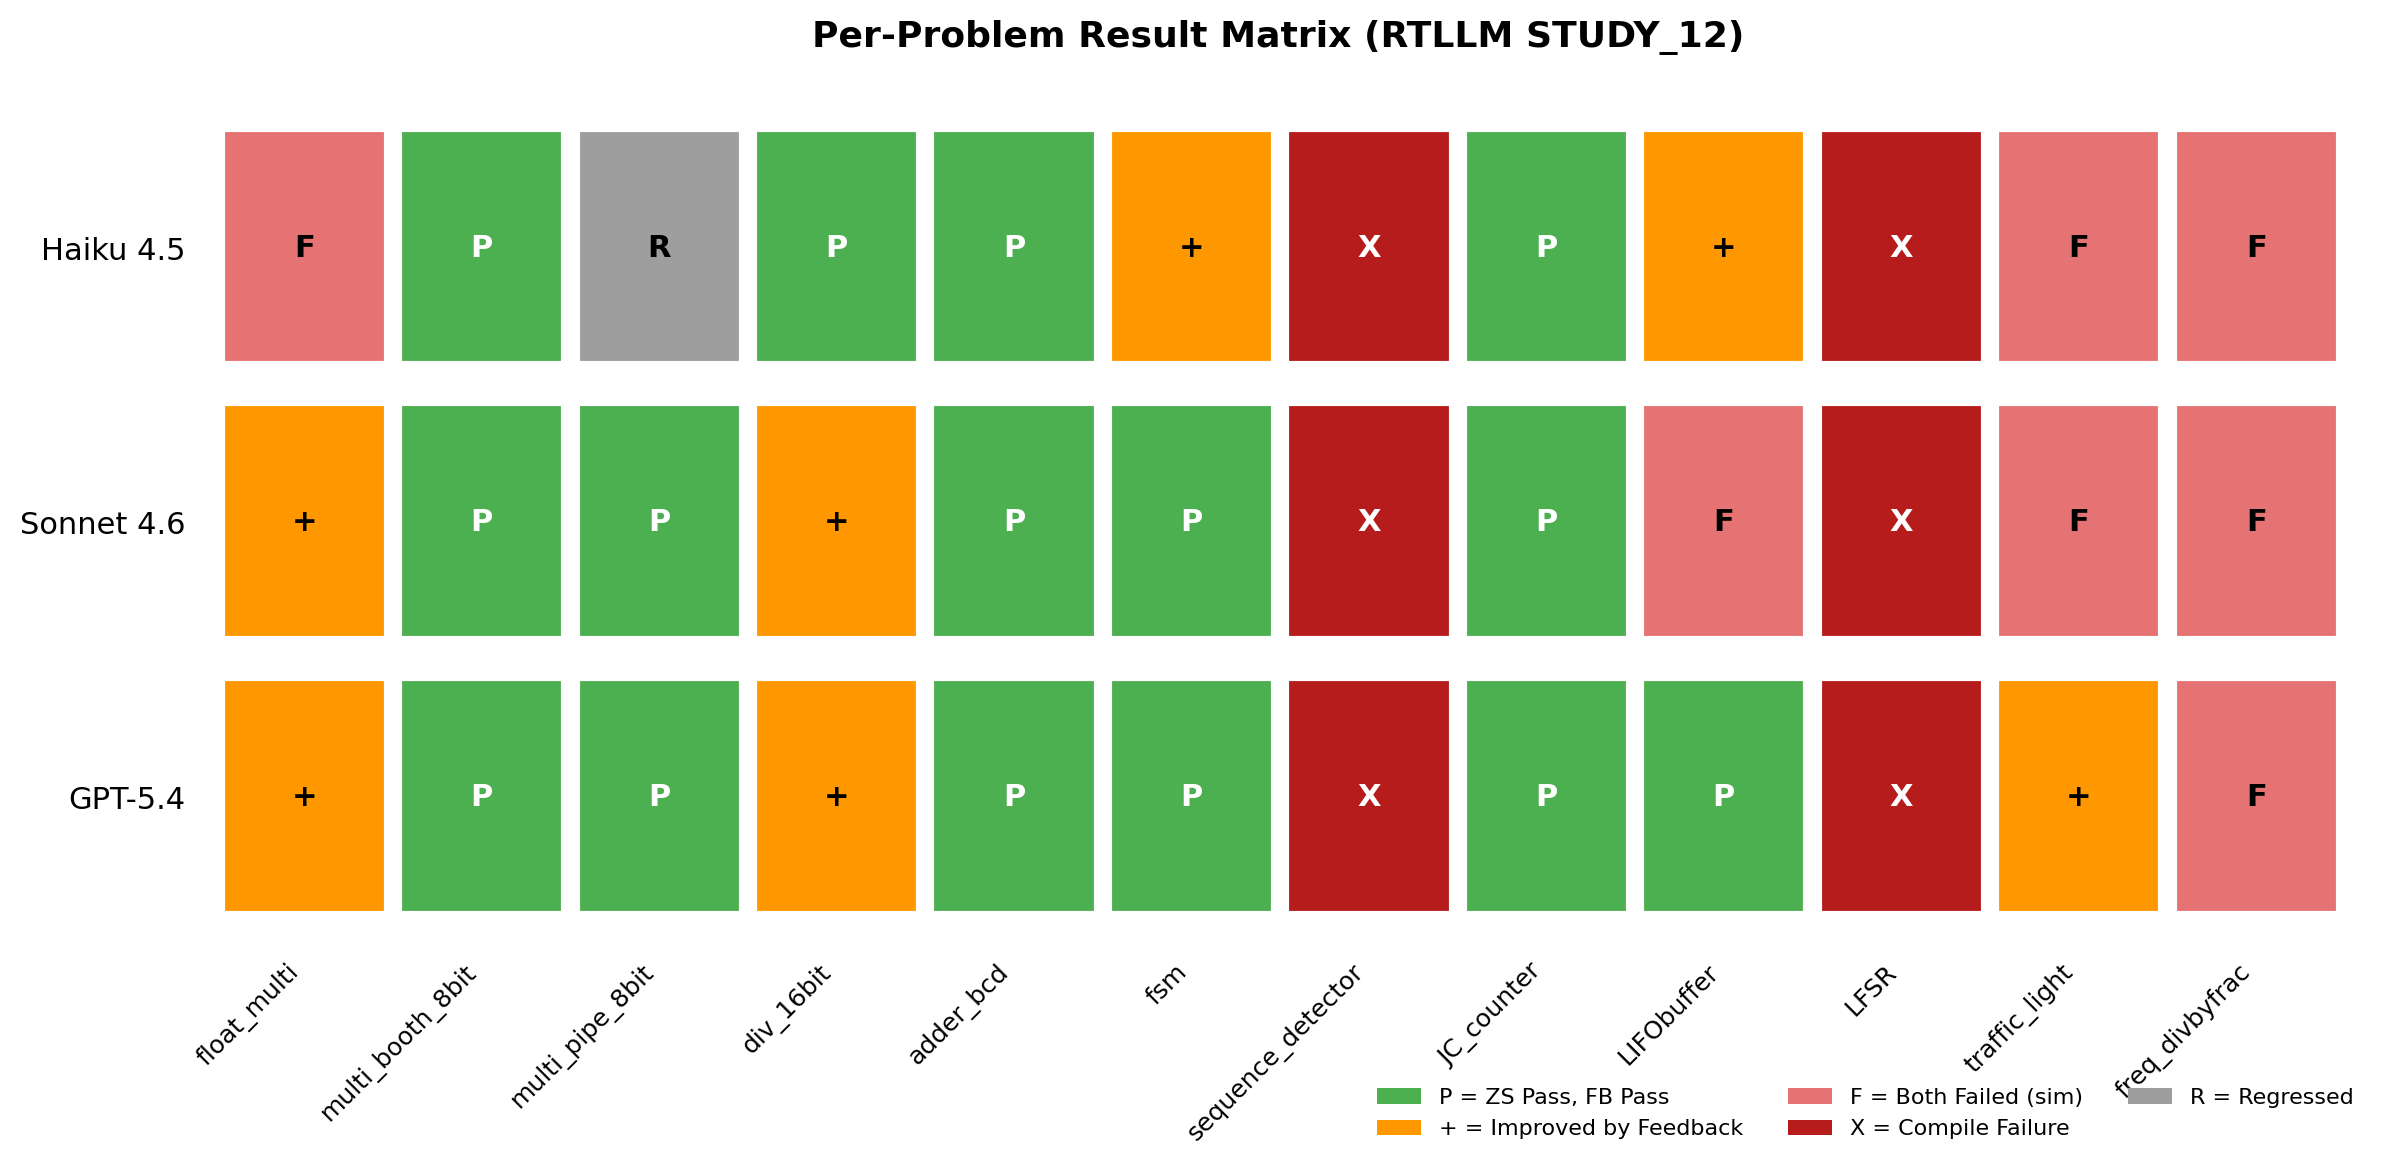
\includegraphics[width=0.85\textwidth]{figure/fig_per_problem_matrix.png}
\caption{RTLLM\_STUDY\_12逐题结果矩阵}
\label{fig:per_problem_matrix}
\end{figure}

\subsection{关键发现}

反馈对所有模型均有正向增益，验证了反馈循环在更难benchmark上的基础有效性。值得注意的是，强模型从反馈中获益最大——GPT-5.4的增益（+33个百分点）远超Sonnet（+17个百分点）和Haiku（+8个百分点）。这表明并非弱模型最需要反馈，而是强模型最能利用反馈。

实验还发现存在仅反馈可解的题目：GPT-5.4的LFSR和traffic\_light在零样本下所有模型均失败，仅在反馈条件下通过。同时存在天花板题：sequence\_detector和freq\_divbyfrac在所有模型和条件下均失败。

\begin{figure}[htbp]
\centering
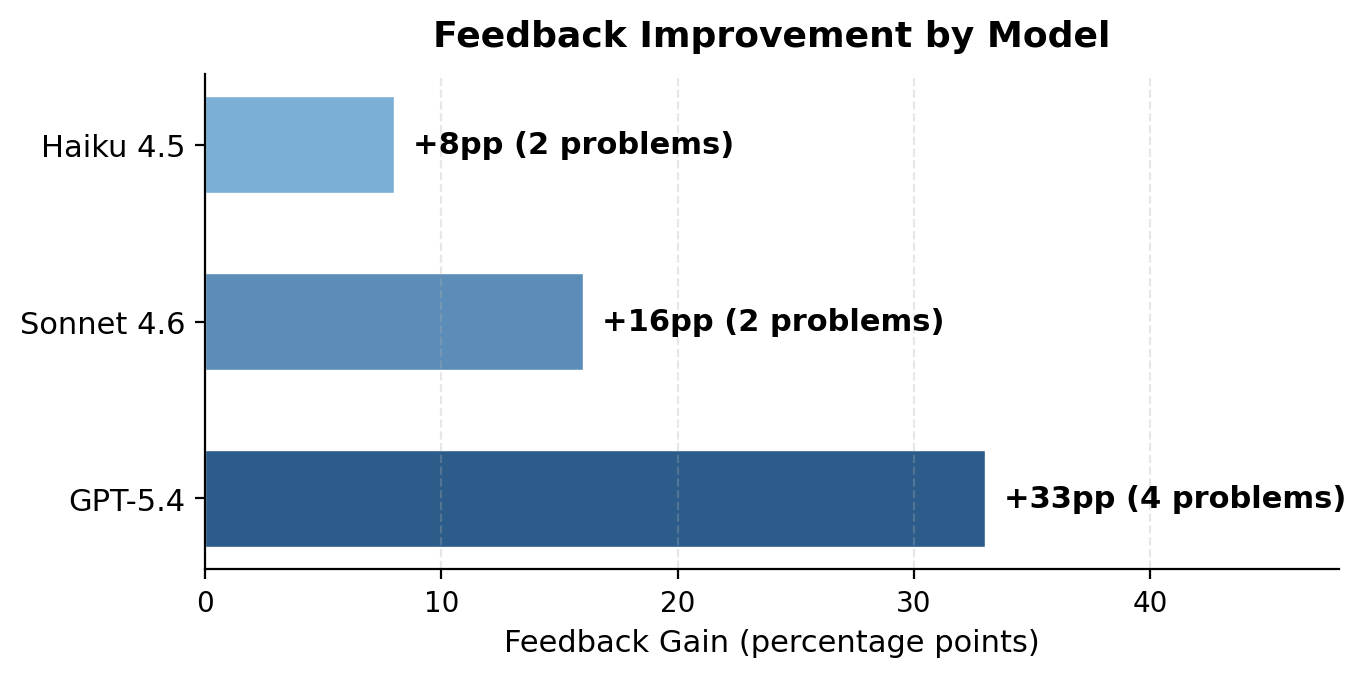
\includegraphics[width=0.7\textwidth]{figure/fig_feedback_gain.png}
\caption{各模型Feedback增益对比}
\label{fig:feedback_gain}
\end{figure}

\section{Feedback vs Retry-only消融实验}

\subsection{实验设计}

为区分反馈循环中"多次重试"与"错误反馈信息"的各自贡献，在GPT-5.4和Sonnet 4.6上运行三条件消融实验（详见第4章）。

\subsection{GPT-5.4消融结果}

% 审阅报告高优先级修改：注明单轮结果与稳定性均值的区别
GPT-5.4的单轮消融结果为：Zero-shot 50\%（6/12），Retry-only 67\%（8/12），Feedback 83\%（10/12）。在该单轮结果中，多采样贡献+17个百分点，反馈信息贡献+16个百分点，反馈信息约占总提升的49\%。需要注意的是，稳定性实验（4轮均值，见\ref{sec:stability}节）修正后的比例为反馈信息约占57\%。

\begin{figure}[htbp]
\centering
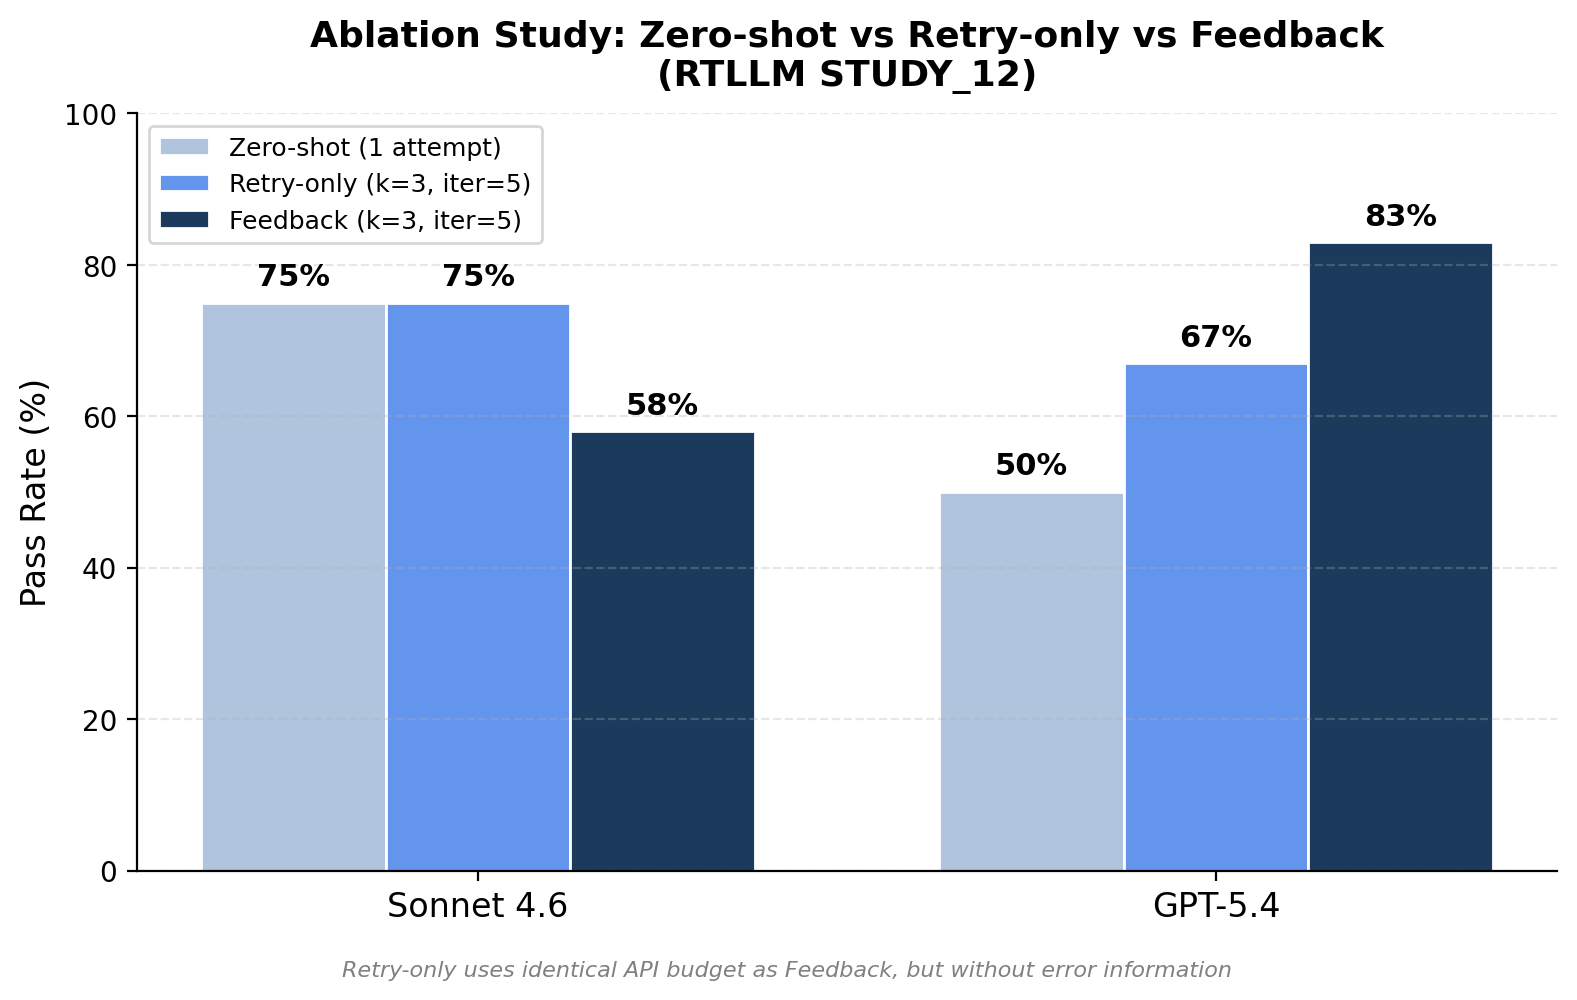
\includegraphics[width=0.7\textwidth]{figure/fig_ablation_comparison.png}
\caption{零样本/重试/反馈三条件对比}
\label{fig:ablation_comparison}
\end{figure}

\subsection{关键证据：仅反馈可解的题目}

% 审阅报告修改："最有力的"改为更稳妥表述
sequence\_detector和traffic\_light在15次独立重试中从未通过，但反馈在2--3轮内成功修复。这为错误反馈信息提供了独立采样无法获得的修复信号提供了直接证据。

\begin{figure}[htbp]
\centering
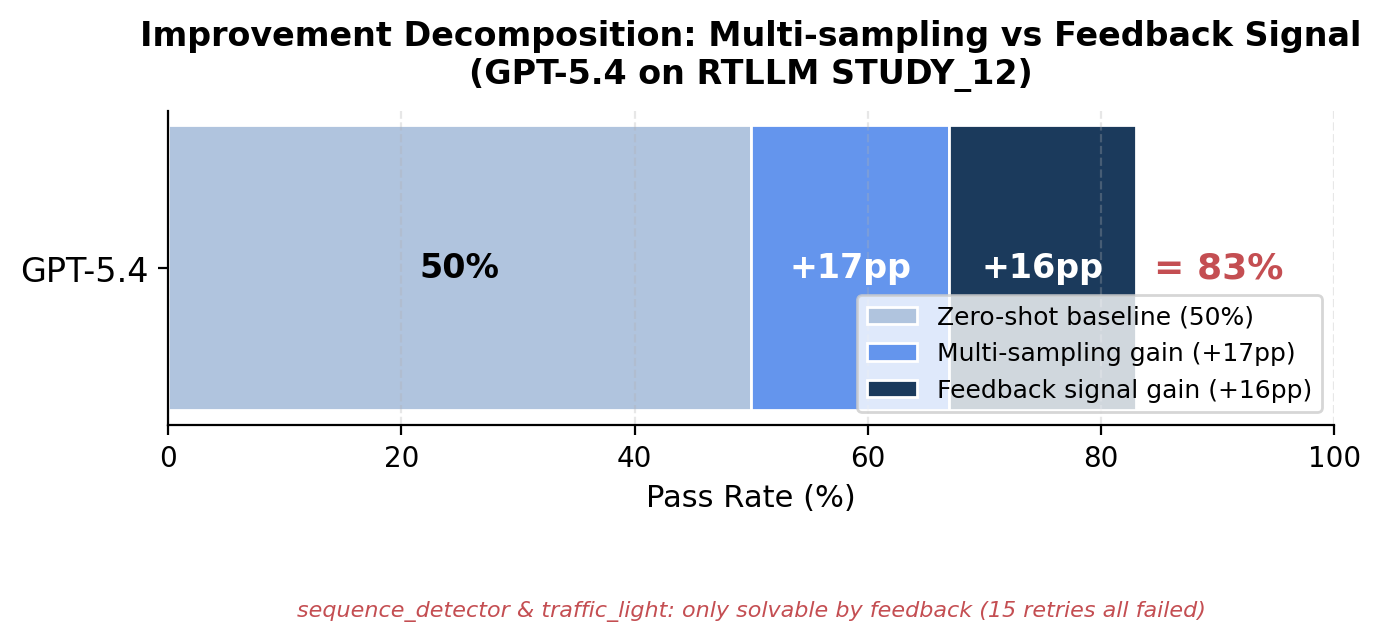
\includegraphics[width=0.7\textwidth]{figure/fig_ablation_decomposition.png}
\caption{GPT-5.4反馈收益来源分解}
\label{fig:ablation_decomposition}
\end{figure}

\subsection{Sonnet消融结果}

Sonnet 4.6的单轮消融结果显示Feedback（58\%）低于Retry-only（75\%），但该结果受单轮随机波动影响较大。Sonnet的消融结论需要结合稳定性实验综合判断。

\section{稳定性重复实验}
\label{sec:stability}

\subsection{GPT-5.4稳定性结果}

\begin{table}[htbp]
\centering
\caption{GPT-5.4稳定性实验统计}
\label{tab:gpt_stability}
\begin{tabular}{lrrr}
\toprule
统计量 & Zero-shot & Retry-only & Feedback \\
\midrule
均值 & 50.0\% & 62.5\% & 79.2\% \\
标准差 & $\pm$11.8\% & $\pm$4.2\% & $\pm$4.2\% \\
FB>RO轮次 & — & — & 4/4 \\
\bottomrule
\end{tabular}
\end{table}

在4轮独立重复中，Feedback始终优于Retry-only，且无一例外。反馈不仅提升了平均通过率，还将标准差从11.8\%（零样本）压缩至4.2\%。

\begin{figure}[htbp]
\centering
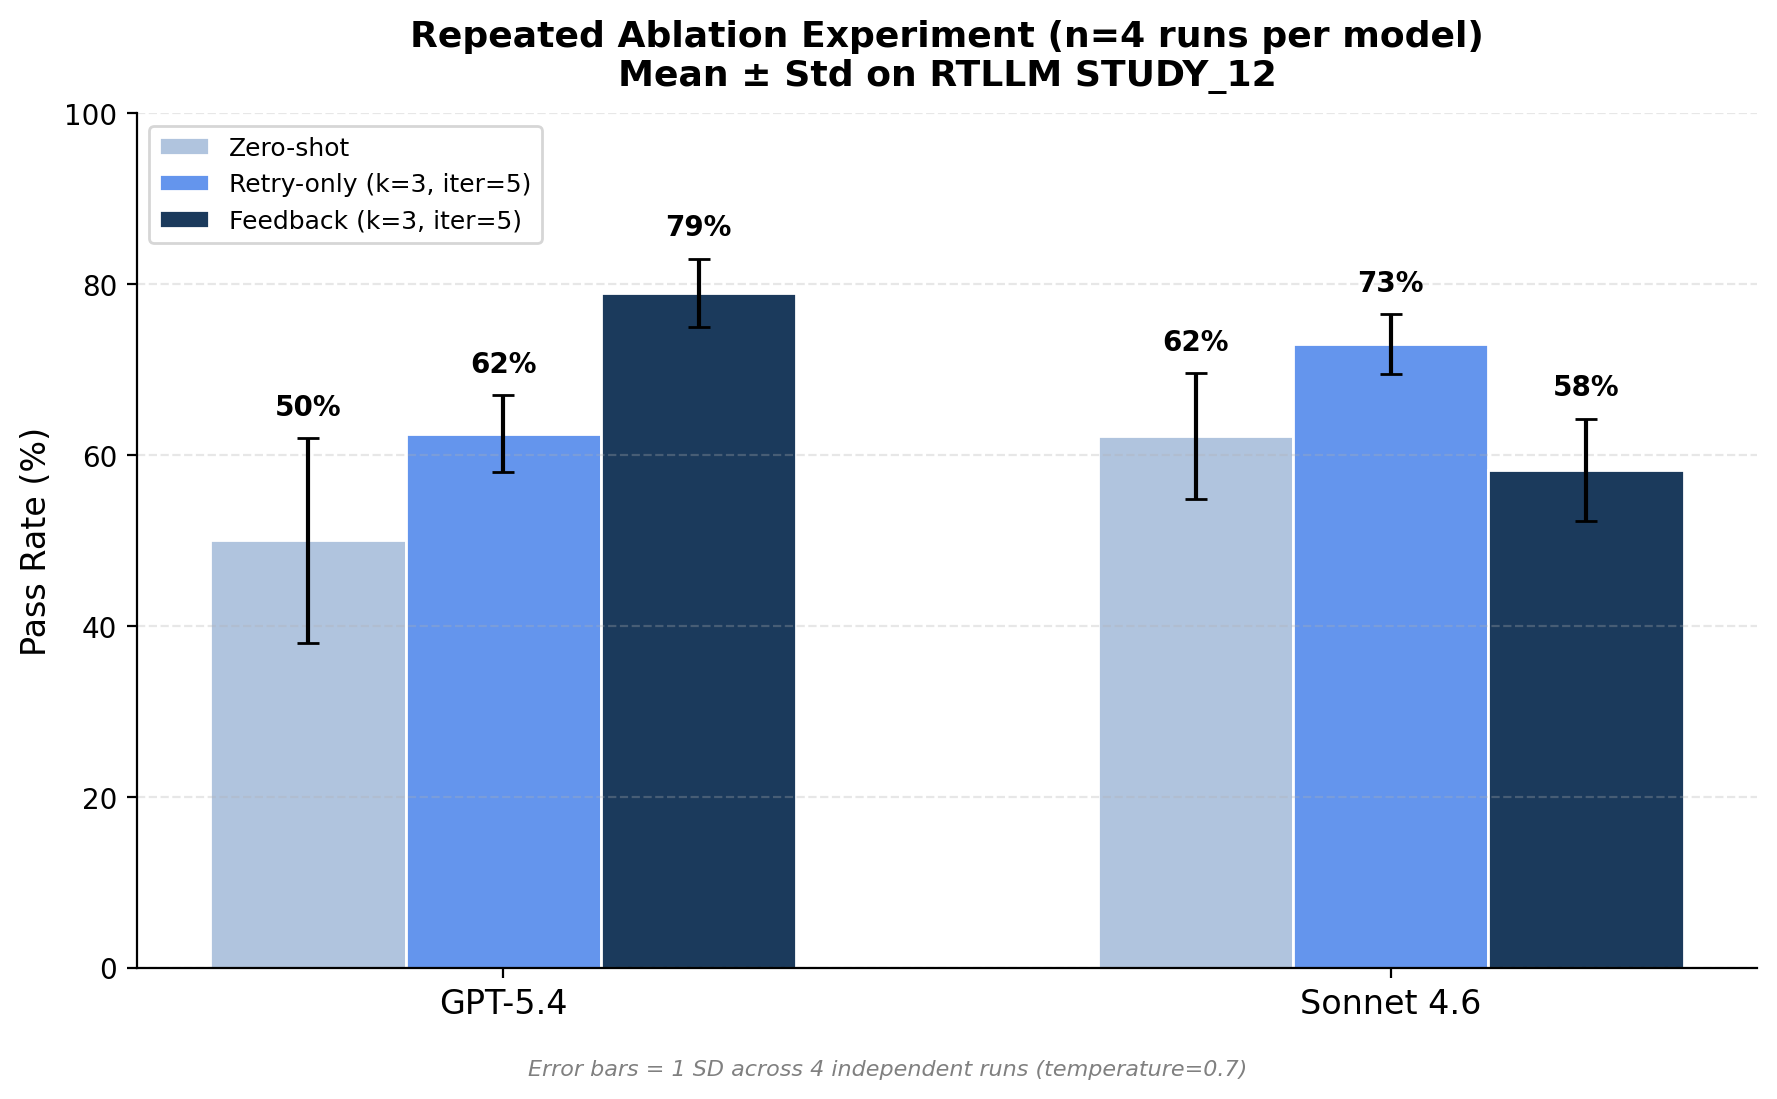
\includegraphics[width=0.7\textwidth]{figure/fig_stability_ablation.png}
\caption{稳定性实验三条件均值与标准差}
\label{fig:stability_ablation}
\end{figure}

\subsection{Sonnet 4.6稳定性结果}

\begin{table}[htbp]
\centering
\caption{Sonnet 4.6稳定性实验统计}
\label{tab:sonnet_stability}
\begin{tabular}{lrrr}
\toprule
统计量 & Zero-shot & Retry-only & Feedback \\
\midrule
均值 & 62.5\% & 72.9\% & 58.3\% \\
标准差 & $\pm$7.2\% & $\pm$3.6\% & $\pm$5.9\% \\
FB>RO轮次 & — & — & 0/4 \\
\bottomrule
\end{tabular}
\end{table}

Sonnet上Feedback低于Retry-only的结论在4轮中稳定成立。

\begin{figure}[htbp]
\centering
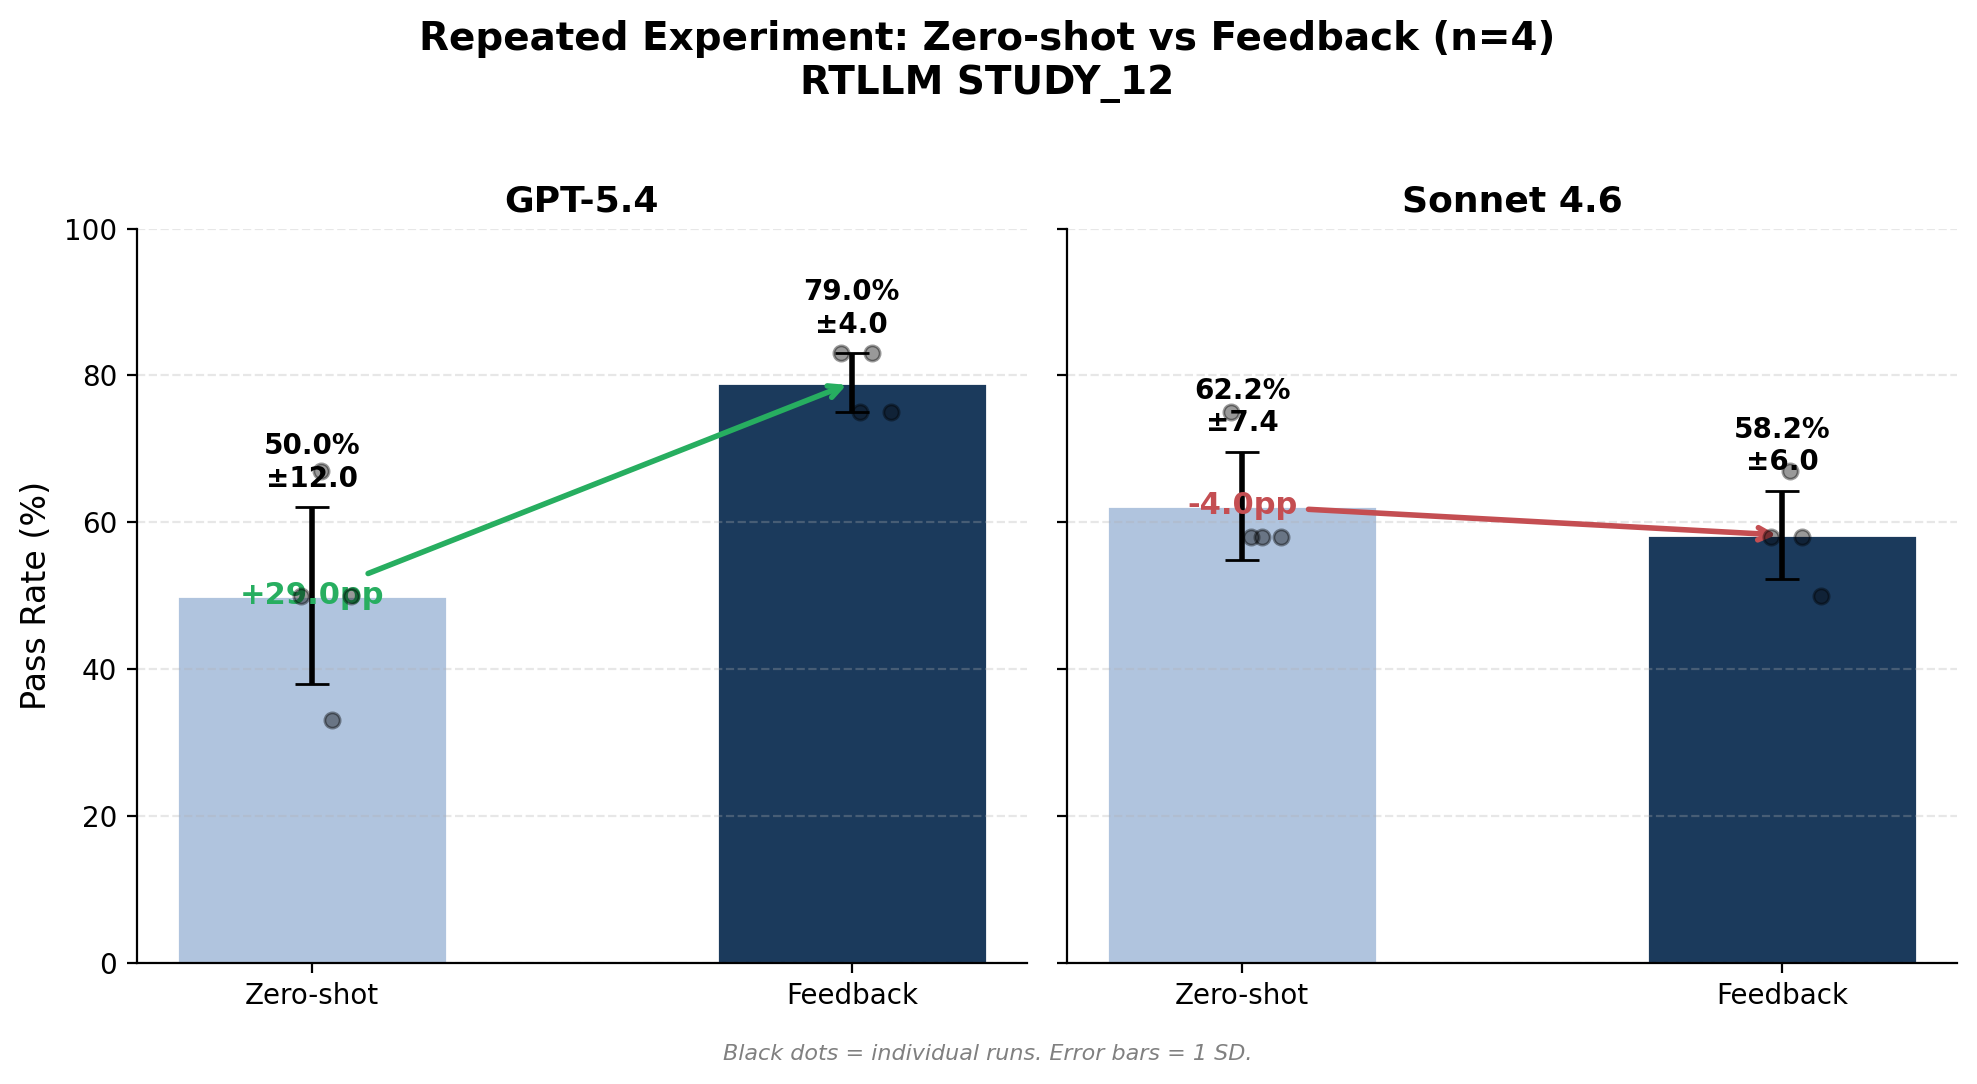
\includegraphics[width=0.7\textwidth]{figure/fig_stability_formal.png}
\caption{正式实验重复结果对比}
\label{fig:stability_formal}
\end{figure}

\subsection{模型依赖性分析}

GPT-5.4与Sonnet 4.6对反馈的响应截然相反：GPT-5.4上FB相对RO的增益为+16.7个百分点，Sonnet上为$-$14.6个百分点。这一两极分化结果在4轮重复中完全稳定，说明反馈机制的有效性具有模型依赖性。

\section{反馈粒度实验}

\subsection{总体结果}

\begin{table}[htbp]
\centering
\caption{反馈粒度实验通过率}
\label{tab:granularity}
\begin{tabular}{lrr}
\toprule
级别 & GPT-5.4 & Sonnet 4.6 \\
\midrule
L0 Zero-shot & 58\% (7/12) & 50\% (6/12) \\
L1 Retry-only & 75\% (9/12) & 67\% (8/12) \\
L2 Compile-only & \textbf{92\%} (11/12) & \textbf{75\%} (9/12) \\
L3 Succinct & \textbf{92\%} (11/12) & 67\% (8/12) \\
L4 Rich & 83\% (10/12) & 67\% (8/12) \\
\bottomrule
\end{tabular}
\end{table}

\begin{figure}[htbp]
\centering
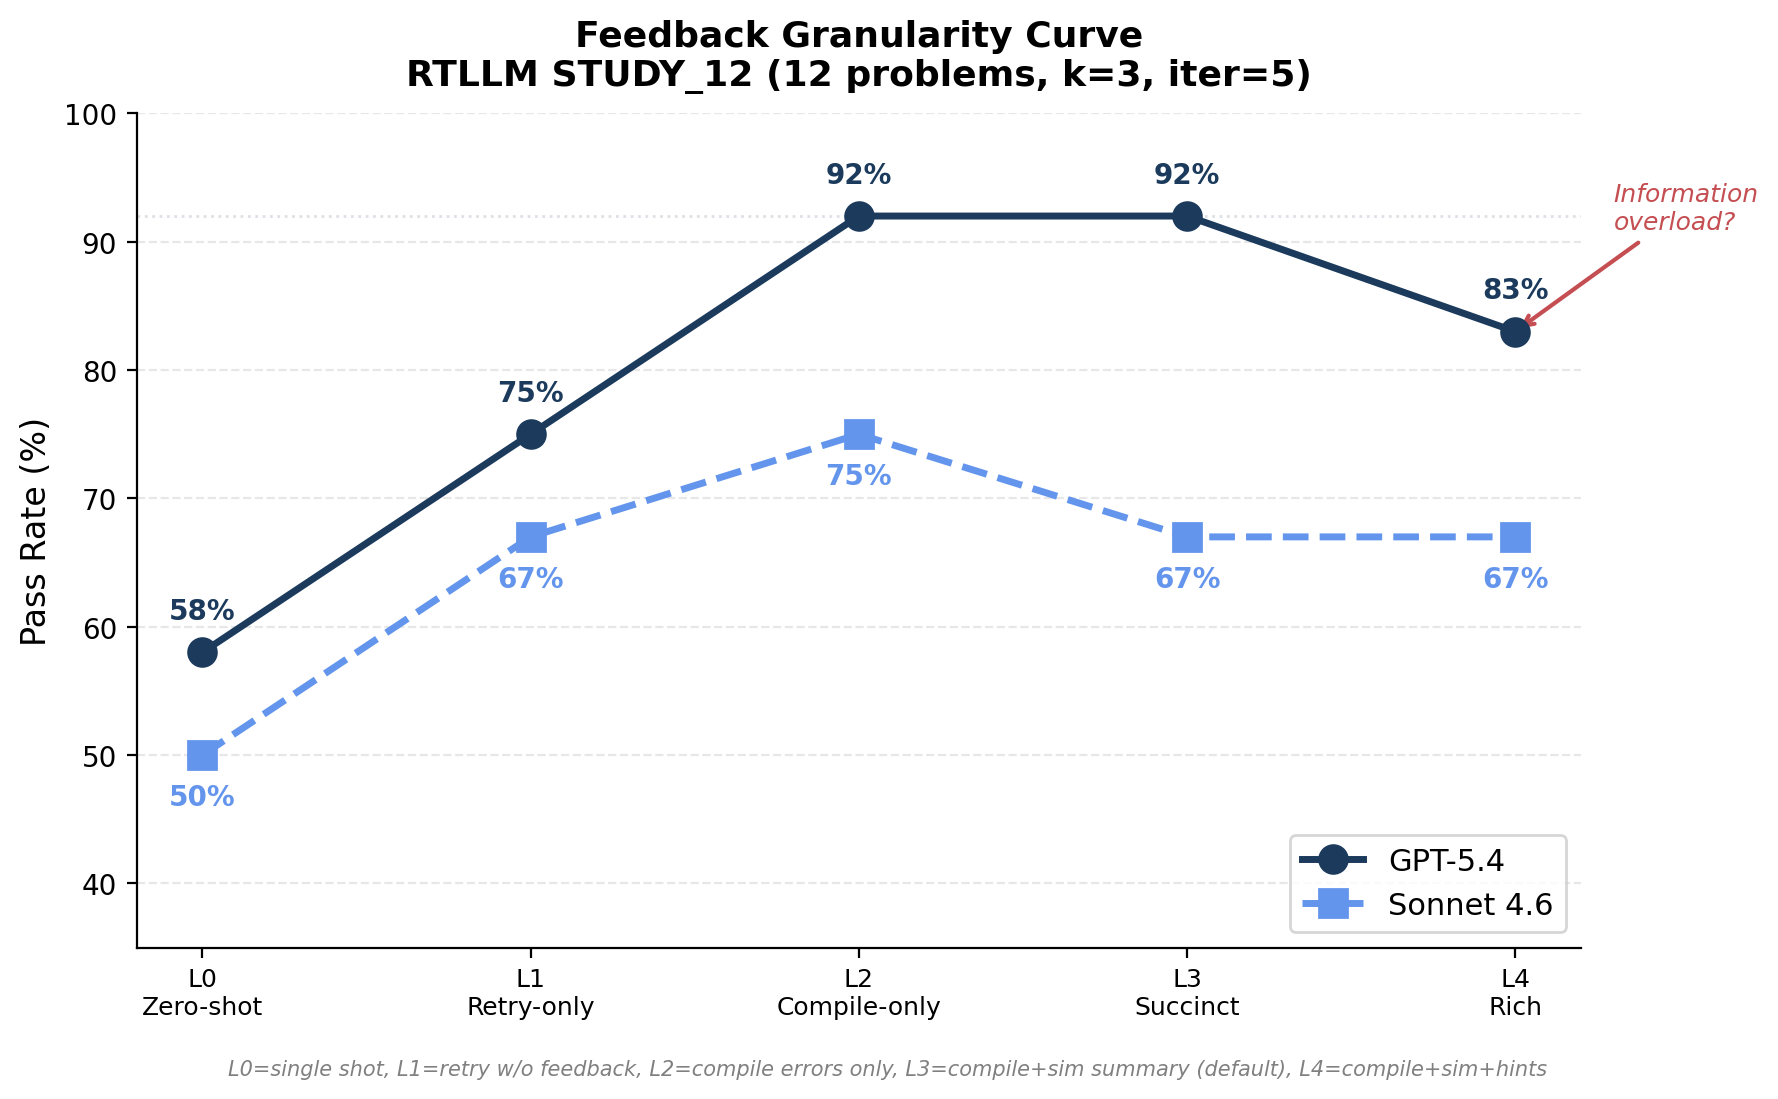
\includegraphics[width=0.7\textwidth]{figure/fig_granularity_curve.png}
\caption{反馈粒度通过率曲线（倒U型）}
\label{fig:granularity_curve}
\end{figure}

\subsection{倒U型趋势}

实验结果呈现出"倒U型"趋势：通过率随反馈信息量的增加先升后降。L2和L3达到峰值，而L4反而出现下降。

\begin{figure}[htbp]
\centering
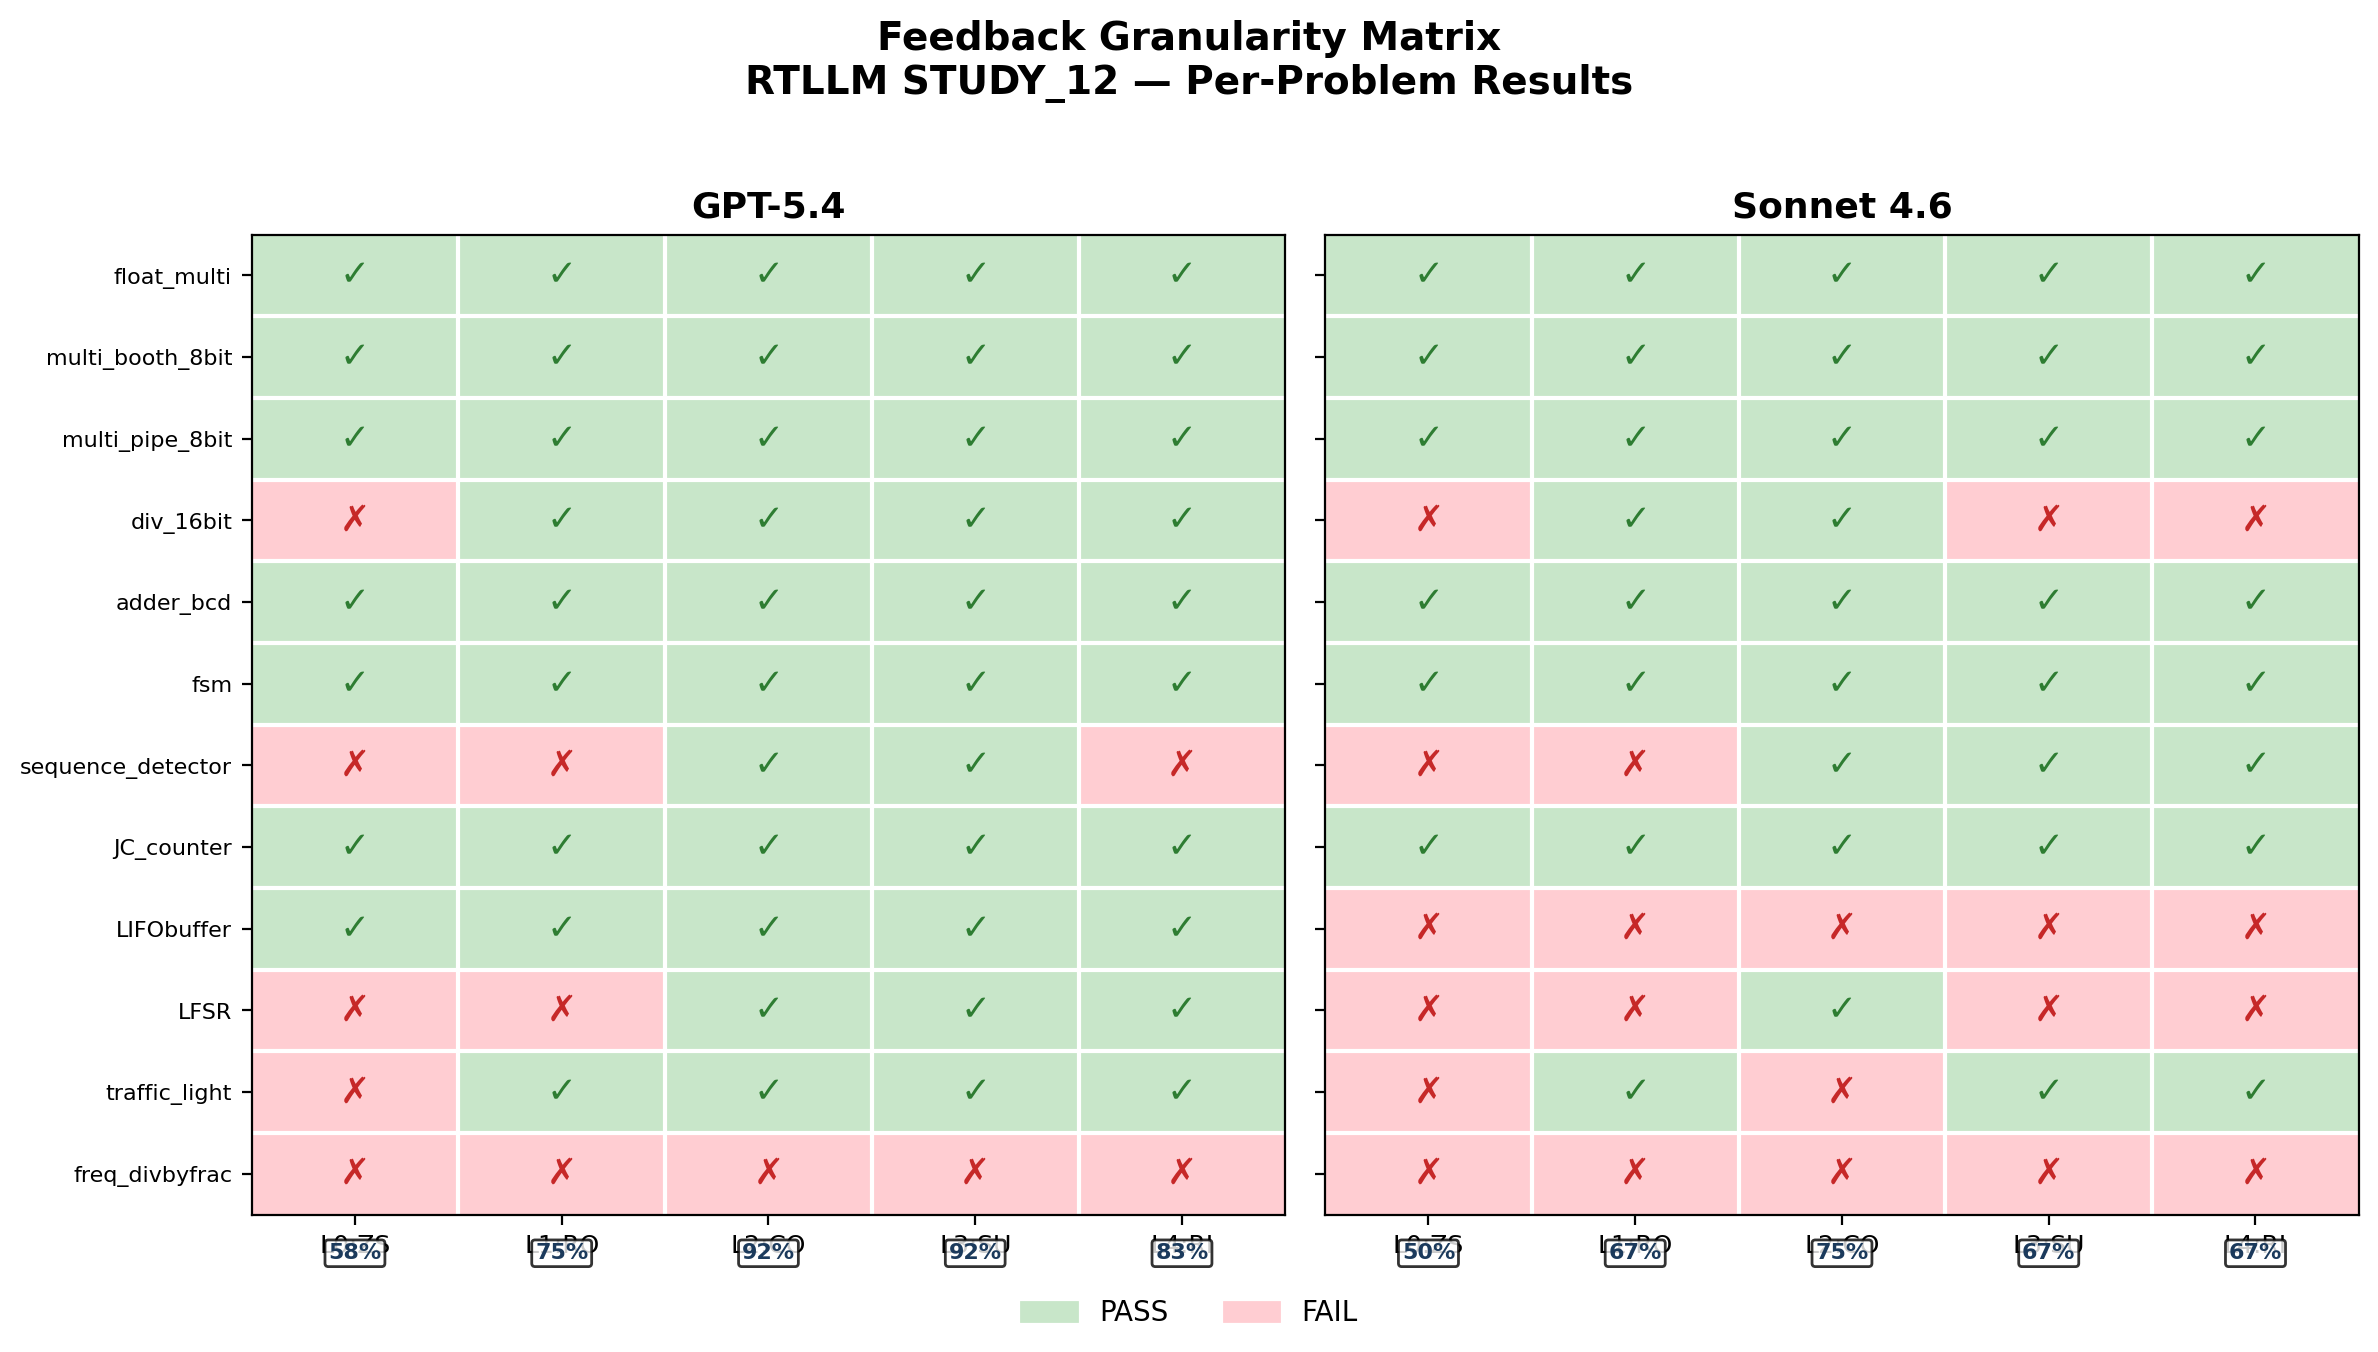
\includegraphics[width=0.85\textwidth]{figure/fig_granularity_matrix.png}
\caption{反馈粒度逐题结果矩阵}
\label{fig:granularity_matrix}
\end{figure}

\subsection{编译反馈的高效性}

L1$\rightarrow$L2是最大的跃升点，表明即使是最基础的编译错误反馈也具有极高的修复价值。L2 Compile-only在两个模型上均为最优或并列最优，是最稳健的通用选择。

\section{多轮对话反馈实验}

\subsection{实验说明}

本节报告的多轮对话反馈结果均来自v2修正版。v1版本因反馈数据源bug已在权威实验索引中标记为Superseded。

\subsection{GPT-5.4结果}

\begin{table}[htbp]
\centering
\caption{多轮对话反馈v2实验结果（GPT-5.4）}
\label{tab:mt_gpt}
\begin{tabular}{lr}
\toprule
条件 & 通过率 \\
\midrule
A: ST $k$=3 & 83\% (5/6) \\
D: ST $k$=1 & 83\% (5/6) \\
B: MT $k$=1 & 100\% (5/5)$^*$ \\
C: CO $k$=3 & 83\% (5/6) \\
\bottomrule
\end{tabular}
\\[4pt]
\small $^*$freq\_divbyfrac因API超时排除。
\end{table}

\subsection{Sonnet 4.6结果}

\begin{table}[htbp]
\centering
\caption{多轮对话反馈v2实验结果（Sonnet 4.6）}
\label{tab:mt_sonnet}
\begin{tabular}{lr}
\toprule
条件 & 通过率 \\
\midrule
A: ST $k$=3 & 17\% (1/6) \\
D: ST $k$=1 & 33\% (2/6) \\
B: MT $k$=1 & 50\% (3/6) \\
C: CO $k$=3 & 33\% (2/6) \\
\bottomrule
\end{tabular}
\end{table}

\begin{figure}[htbp]
\centering
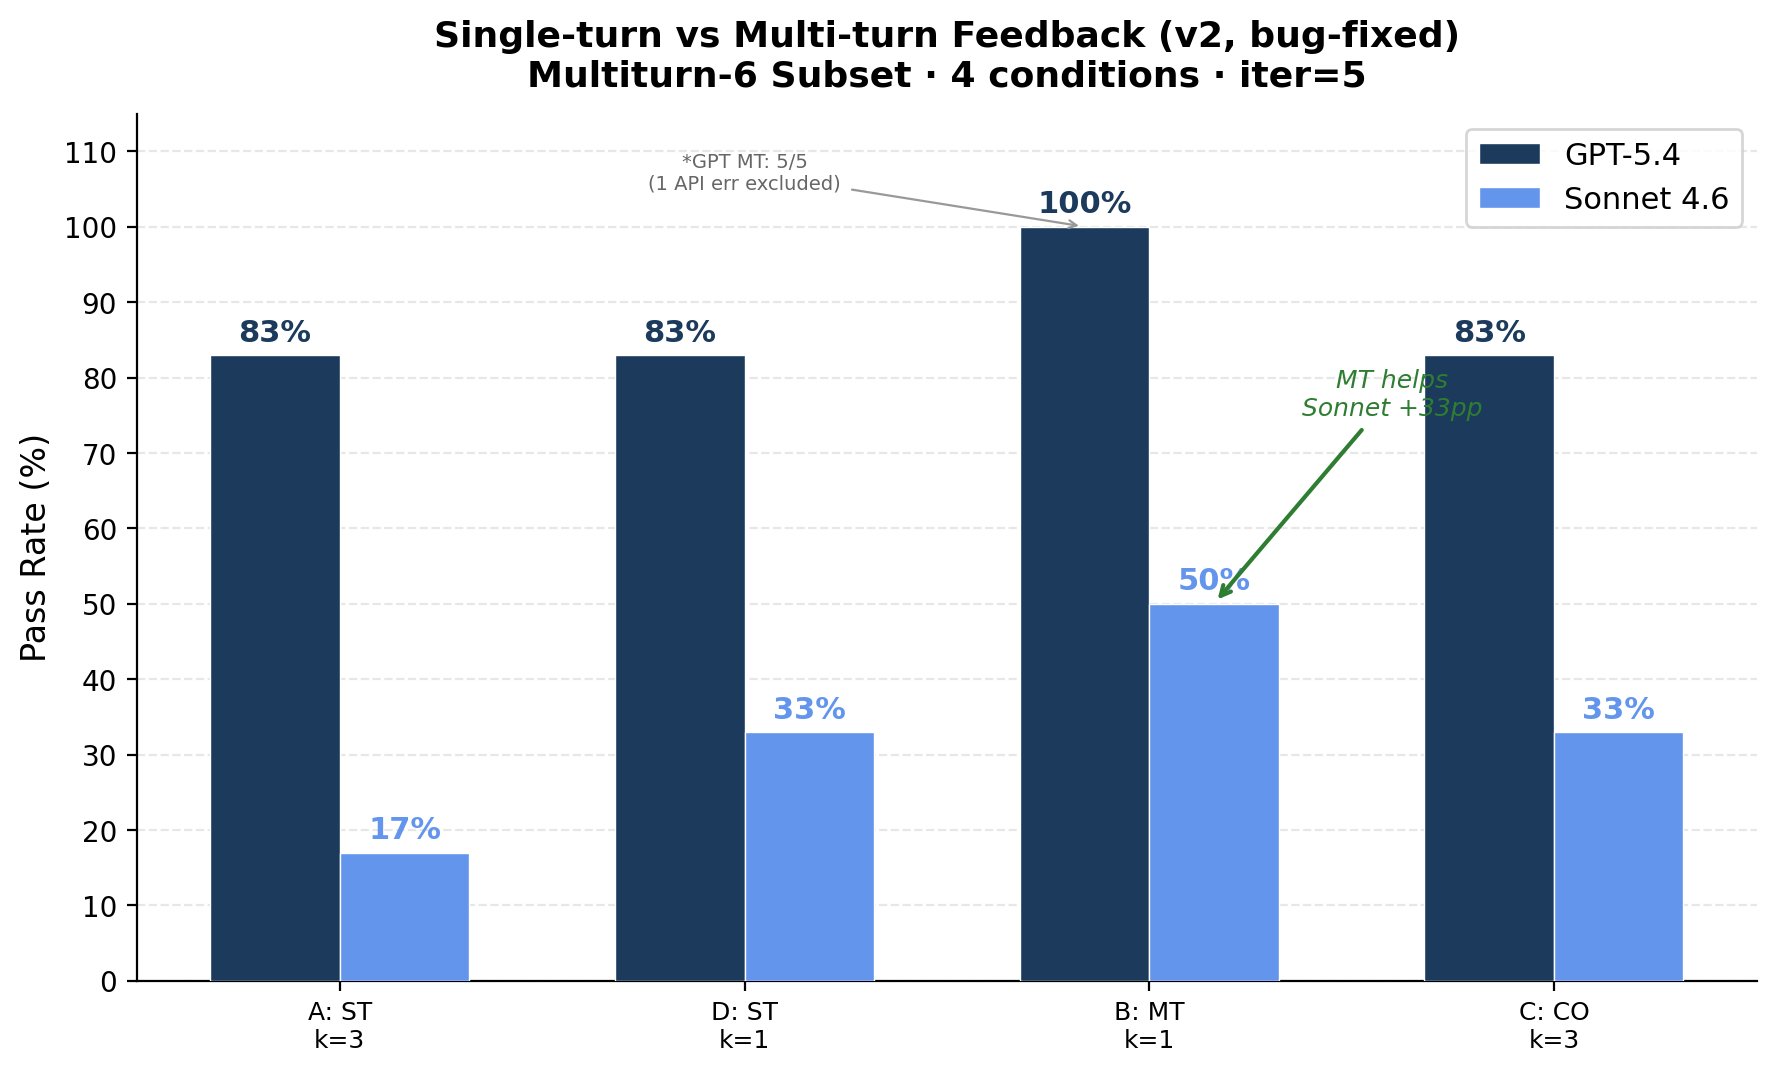
\includegraphics[width=0.7\textwidth]{figure/fig_multiturn_comparison_v2.png}
\caption{多轮对话反馈v2条件对比}
\label{fig:multiturn_comparison}
\end{figure}

\begin{figure}[htbp]
\centering
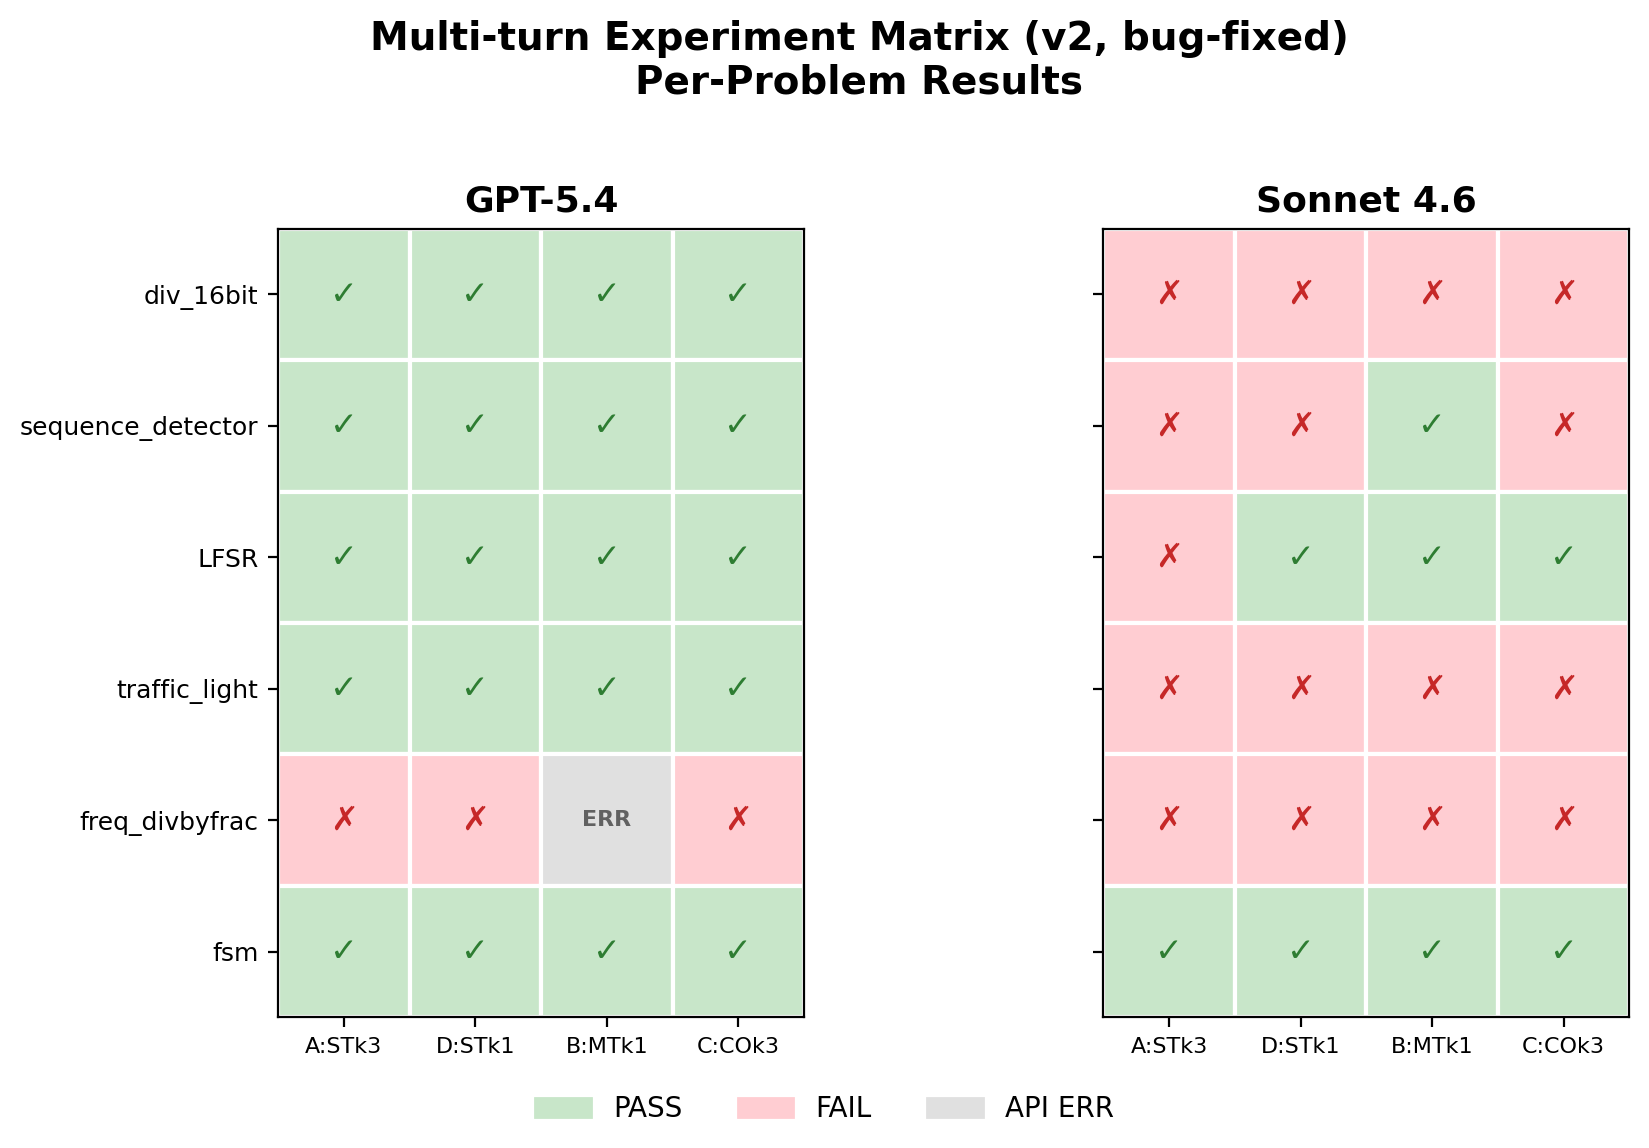
\includegraphics[width=0.85\textwidth]{figure/fig_multiturn_matrix_v2.png}
\caption{多轮对话反馈v2逐题矩阵}
\label{fig:multiturn_matrix}
\end{figure}

\subsection{分析}

多轮对话模式在两个模型上均表现出优势（+17个百分点），表明持续的对话上下文有助于模型理解修复历史。但该实验在6题子集上进行且为单次运行，结论需谨慎表述。

\section{提示词策略实验}

\subsection{总体结果}

使用GPT-5.4在STUDY\_12上对比四种提示策略，结果如表\ref{tab:prompt_strategy}所示。

\begin{table}[htbp]
\centering
\caption{提示词策略实验结果（GPT-5.4）}
\label{tab:prompt_strategy}
\begin{tabular}{lrrr}
\toprule
策略 & Zero-shot & Feedback & FB增益 \\
\midrule
P0: Base & 58\% (7/12) & 92\% (11/12) & +34pp \\
P1: CoT & 50\% (6/12) & 92\% (11/12) & +42pp \\
P2: Few-shot & \textbf{67\%} (8/12) & 92\% (11/12) & +25pp \\
P3: Few-shot+CoT & 58\% (7/12) & 92\% (11/12) & +34pp \\
\bottomrule
\end{tabular}
\end{table}

\begin{figure}[htbp]
\centering
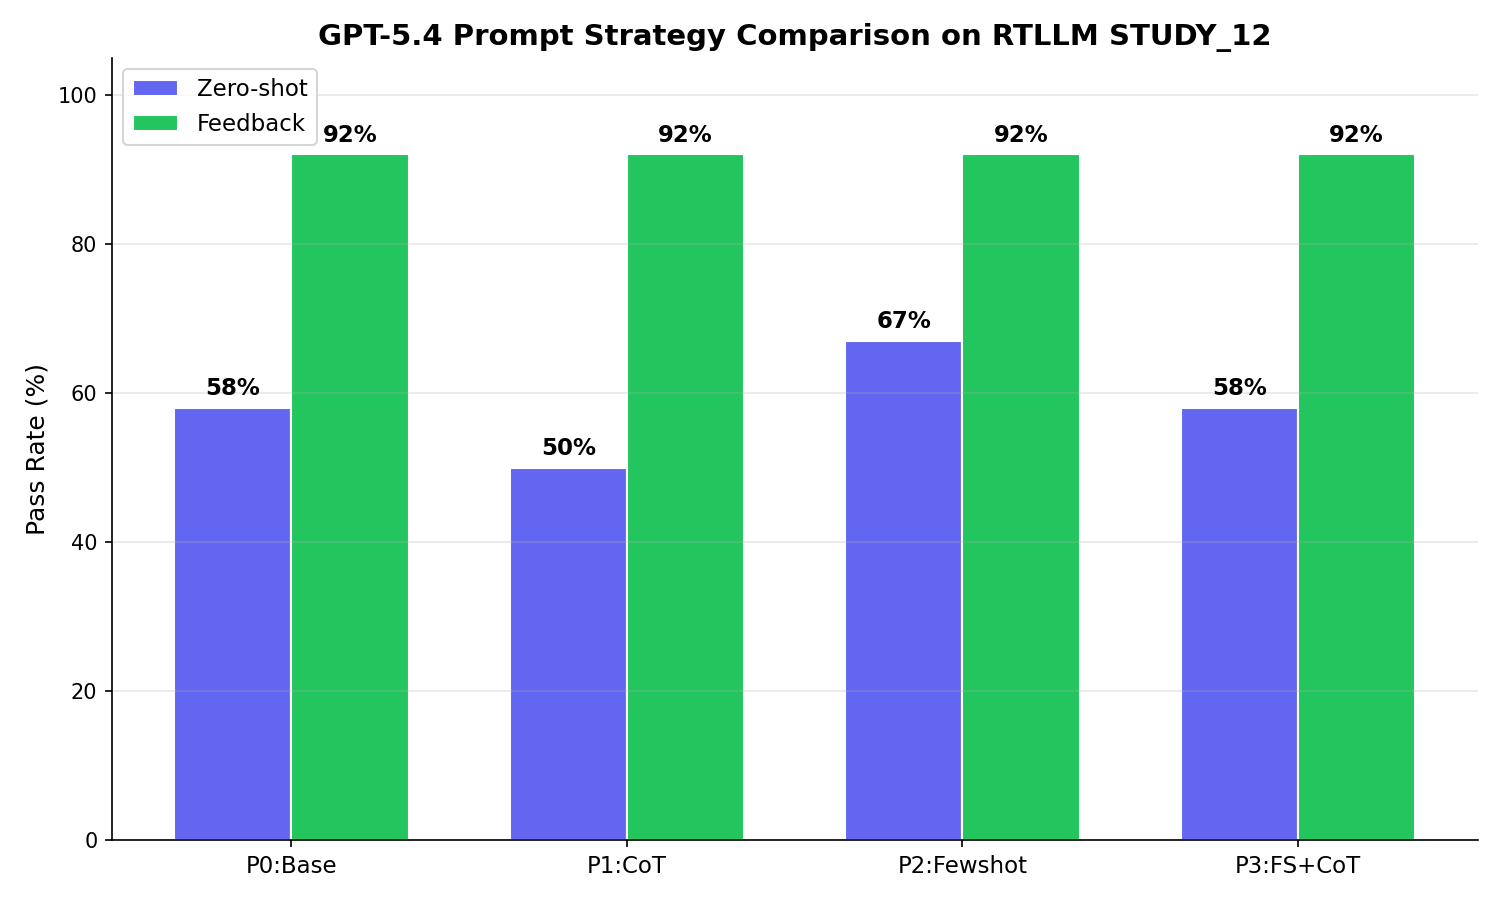
\includegraphics[width=0.7\textwidth]{figure/fig_prompt_strategy_comparison.png}
\caption{提示词策略零样本与反馈对比}
\label{fig:prompt_strategy_comparison}
\end{figure}

\subsection{Zero-shot阶段的策略差异}

Few-shot（P2）是零样本最优策略（67\%），相比Base（P0）提升+9个百分点。CoT（P1）反而略有负面影响（50\%，$-$8个百分点）。

\subsection{Feedback的"拉平效应"}

四种策略在引入反馈后全部收敛至92\%（11/12），仅freq\_divbyfrac在所有策略下均未通过。这一"拉平效应"表明：反馈循环是代码质量的主导因素，初始提示词策略更多影响零样本起点。

\begin{figure}[htbp]
\centering
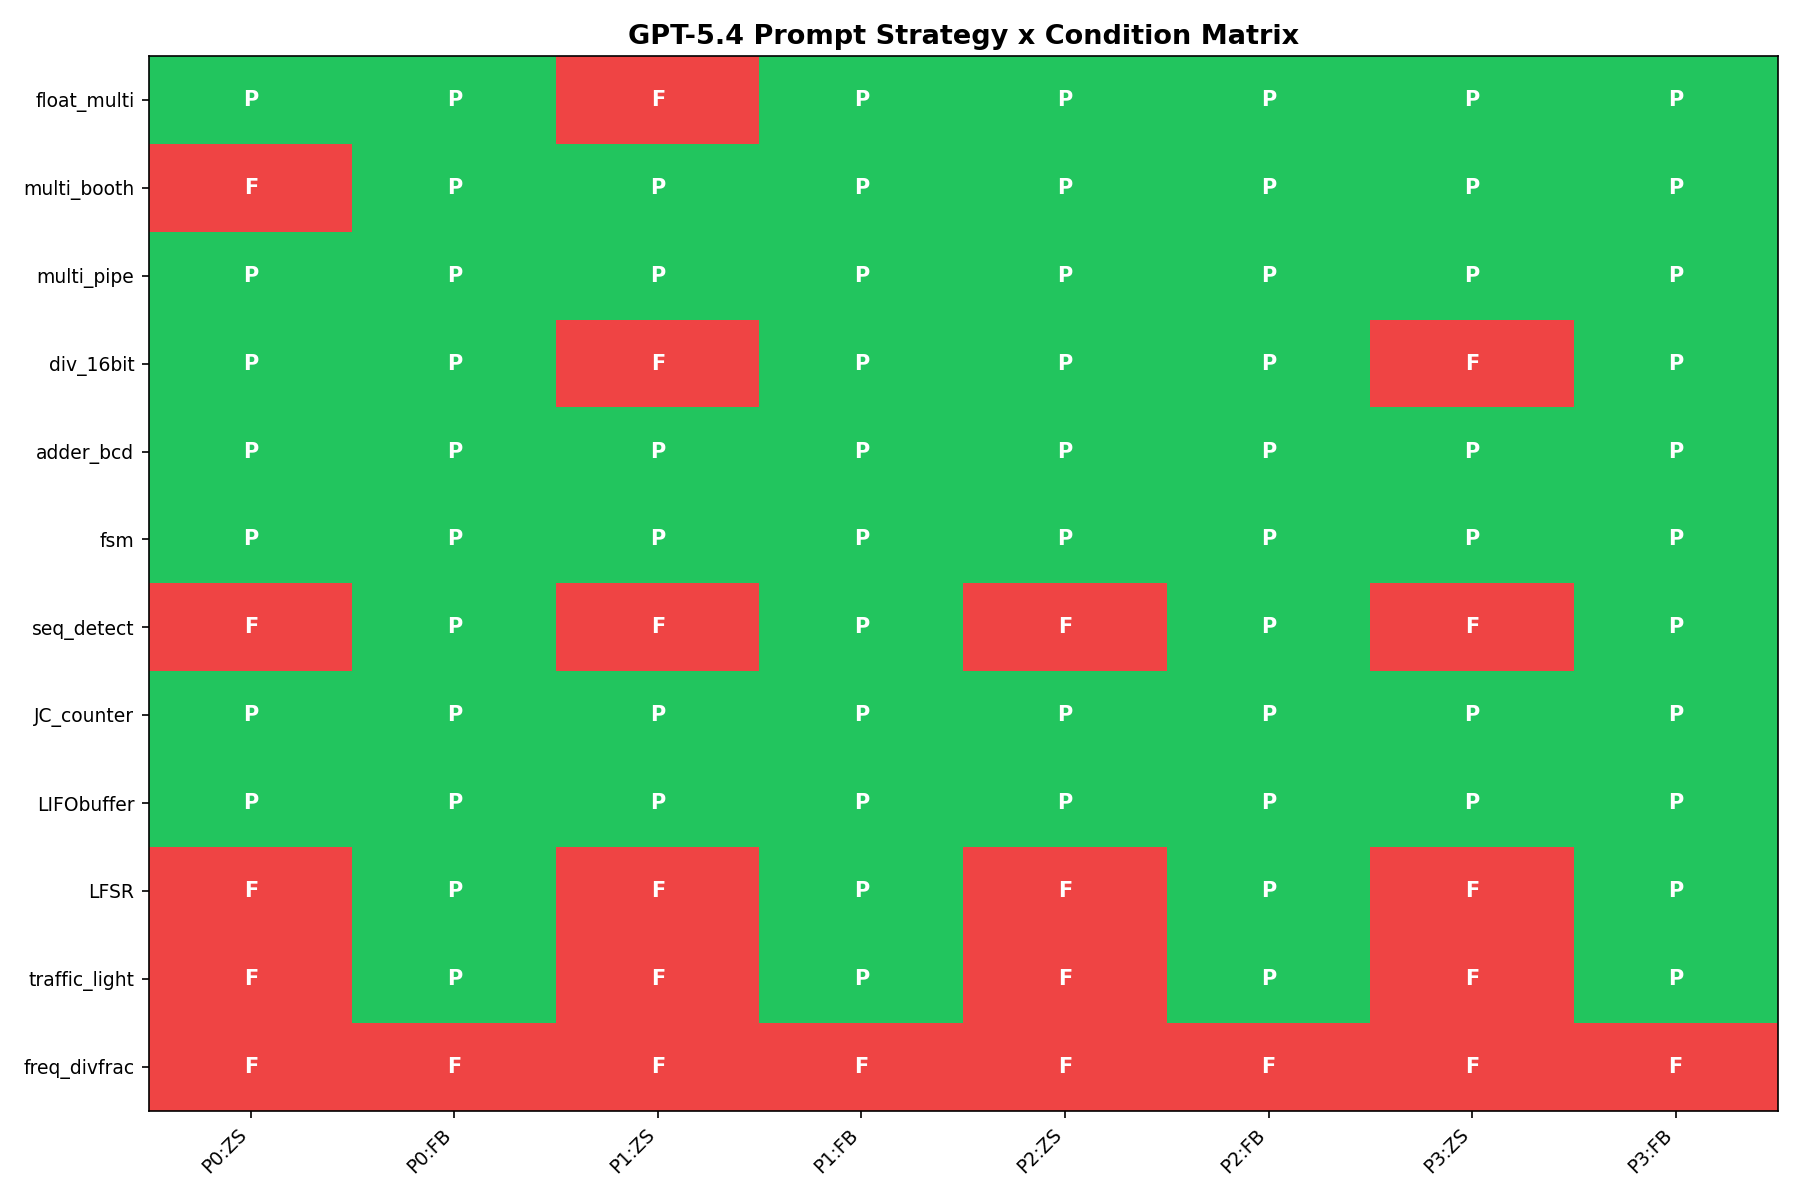
\includegraphics[width=0.85\textwidth]{figure/fig_prompt_strategy_matrix.png}
\caption{提示词策略逐题结果矩阵}
\label{fig:prompt_strategy_matrix}
\end{figure}

\section{典型案例分析}

\subsection{float\_multi：反馈修复最难设计}

float\_multi（IEEE 754浮点乘法器）是STUDY\_12中难度最高的题目。三个模型在零样本下全部失败，但Sonnet和GPT-5.4均在反馈的第1轮迭代中修复成功，而Haiku即使有反馈仍无法修复。

\subsection{LIFObuffer：反馈拉起弱模型}

GPT-5.4零样本即通过，Haiku零样本失败但反馈1轮修复，Sonnet反而无法通过反馈修复。Haiku通过反馈追平了GPT-5.4的零样本水平，说明反馈机制在资源受限场景下提供了"以计算换准确度"的可行路径。

\subsection{天花板题分析}

sequence\_detector在正式实验中所有模型和条件均编译失败，暴露了当前框架的结构性局限。freq\_divbyfrac在所有实验条件下均未通过。值得注意的是，sequence\_detector在后续的消融稳定性实验和提示词策略实验中被成功修复，说明该题并非绝对不可解，而是对初始生成路径敏感。

\section{综合讨论}

\subsection{反馈机制的有效性}

在本文实验设置下，反馈循环在VerilogEval-Human和RTLLM\_STUDY\_12两个benchmark上均表现出正向增益。在RTLLM上，GPT-5.4的增益达到+33个百分点，且该增益在4轮重复实验中稳定存在（79.2\%$\pm$4.2\%）。

\subsection{反馈收益的来源}

消融实验和稳定性实验共同揭示了反馈收益的双重来源：约43\%来自多次采样机会，约57\%来自错误反馈信息本身。后者的独立价值通过"仅反馈可解的题目"得到了证明。

\subsection{模型依赖性}

反馈机制的有效性存在模型依赖性。GPT-5.4上反馈带来稳定的+16.7个百分点增益，而Sonnet 4.6上反馈反而导致$-$14.6个百分点的回退，且这两个结论均在4轮重复中完全稳定。

\subsection{反馈信息量的边界}

在本文实验设置下，粒度实验揭示了一个重要的实践启示：更多的反馈信息并不总是更好。L2 Compile-only是最稳健的通用选择。

\subsection{反馈组织方式与提示词策略}

多轮对话实验（v2）表明持续对话上下文有助于修复。提示词策略实验表明反馈循环将所有策略拉平至92\%，证明反馈是主导修复因素。

\subsection{局限性}

本文实验存在以下局限性：RTLLM\_STUDY\_12仍为12题子集；部分实验为单次运行或小子集，统计效力有限；Sonnet上反馈无效的原因尚未完全明确；天花板题暴露了当前框架对复杂算法生成的局限；实验仅使用Icarus Verilog作为仿真工具。

\section{本章小结}

本章通过七组递进式实验系统验证了AutoChip风格反馈循环的有效性和边界条件。核心结论包括：反馈循环在两个benchmark上均有效，GPT-5.4上增益最大且最稳定；反馈信息贡献约占总提升的57\%；反馈效果具有模型依赖性；反馈信息量存在倒U型边界；多轮对话是有潜力的改进方向；提示词策略与反馈循环为互补关系。
